\documentclass[10pt,twocolumn,letterpaper]{article}
\usepackage[utf8]{inputenc}
\usepackage[T1]{fontenc}
\usepackage{times}
\usepackage{graphicx}
\usepackage{url}
\usepackage{enumitem}
\usepackage{verbatim}
\usepackage[margin=0.75in]{geometry}
\setlist{nosep,leftmargin=*}

\title{\bf AI-Assisted Cryptographic Vulnerability Discovery in an Android APK}
\author{INFO5995 Assignment 1 Team}
\date{}

\begin{document}
\maketitle

\noindent\textbf{Note.} The official USENIX style file is not available in this workspace, so this report uses a two-column LaTeX fallback. The content is ready to move into the official template before final submission if required.

\section*{Introduction}
An APK is the installable package format for Android applications. Auditing an APK usually requires decompilation because the delivered artifact contains compiled bytecode, resources, and the Android manifest rather than directly readable source code. We decompiled \texttt{a1\_case1.apk}, inspected the manifest and key activities, and traced registration, login, session creation, and logout behavior. The main security finding is that the application generates an authentication-related session token with \texttt{java.util.Random}, which is predictable and unsuitable for security-sensitive values.

\section*{System and Threat Model}
The decompiled package name is \texttt{com.example.mastg\_test0016}, with \texttt{MainActivity} as the launcher activity. The app implements local registration, login, and a profile screen. Registration writes plaintext credentials to \texttt{credentials.txt}. Login reads that file, compares the entered username and password, then creates a \texttt{sessionToken} in \texttt{SharedPreferences} under \texttt{SessionPrefs}. The profile screen contains a title, an empty \texttt{WebView}, and a logout button that only removes the token.

Important assets are the username/password pair in \texttt{credentials.txt}, the session token in \texttt{SharedPreferences}, and the authenticated state implied by that token. We assume an attacker can obtain the APK, decompile it, inspect the token generation logic, and observe or trigger login events on a device, emulator, or rooted test environment. The attacker goal is to predict or reconstruct a valid session token and use it to impersonate a logged-in user or bypass intended session integrity guarantees.

\begin{verbatim}
User -> MainActivity -> credentials.txt
User -> Login -> credentials.txt -> sessionToken -> SharedPreferences
User -> Profile -> Log out -> remove(sessionToken)
\end{verbatim}

\section*{How We Found the Vulnerability}
We inspected \texttt{AndroidManifest.xml}, \texttt{MainActivity.java}, \texttt{Login.java}, and \texttt{Profile.java}, then searched the decompiled sources for security-relevant strings and APIs such as ``password'', ``token'', and ``Random''. AI assistance was used to guide the decompilation workflow and sanity-check whether observed random-value generators matched their security role. Two random-value sites were found:
\begin{itemize}
\item \texttt{MainActivity.randomNumberGenerator()}: \texttt{new Random().nextInt(100)}. This appears demo-only.
\item \texttt{Login.generateSessionToken()}: \texttt{new Random()} used to create a 16-character session token. This is security-relevant because it represents authenticated state.
\end{itemize}

\begin{figure}[t]
\centering
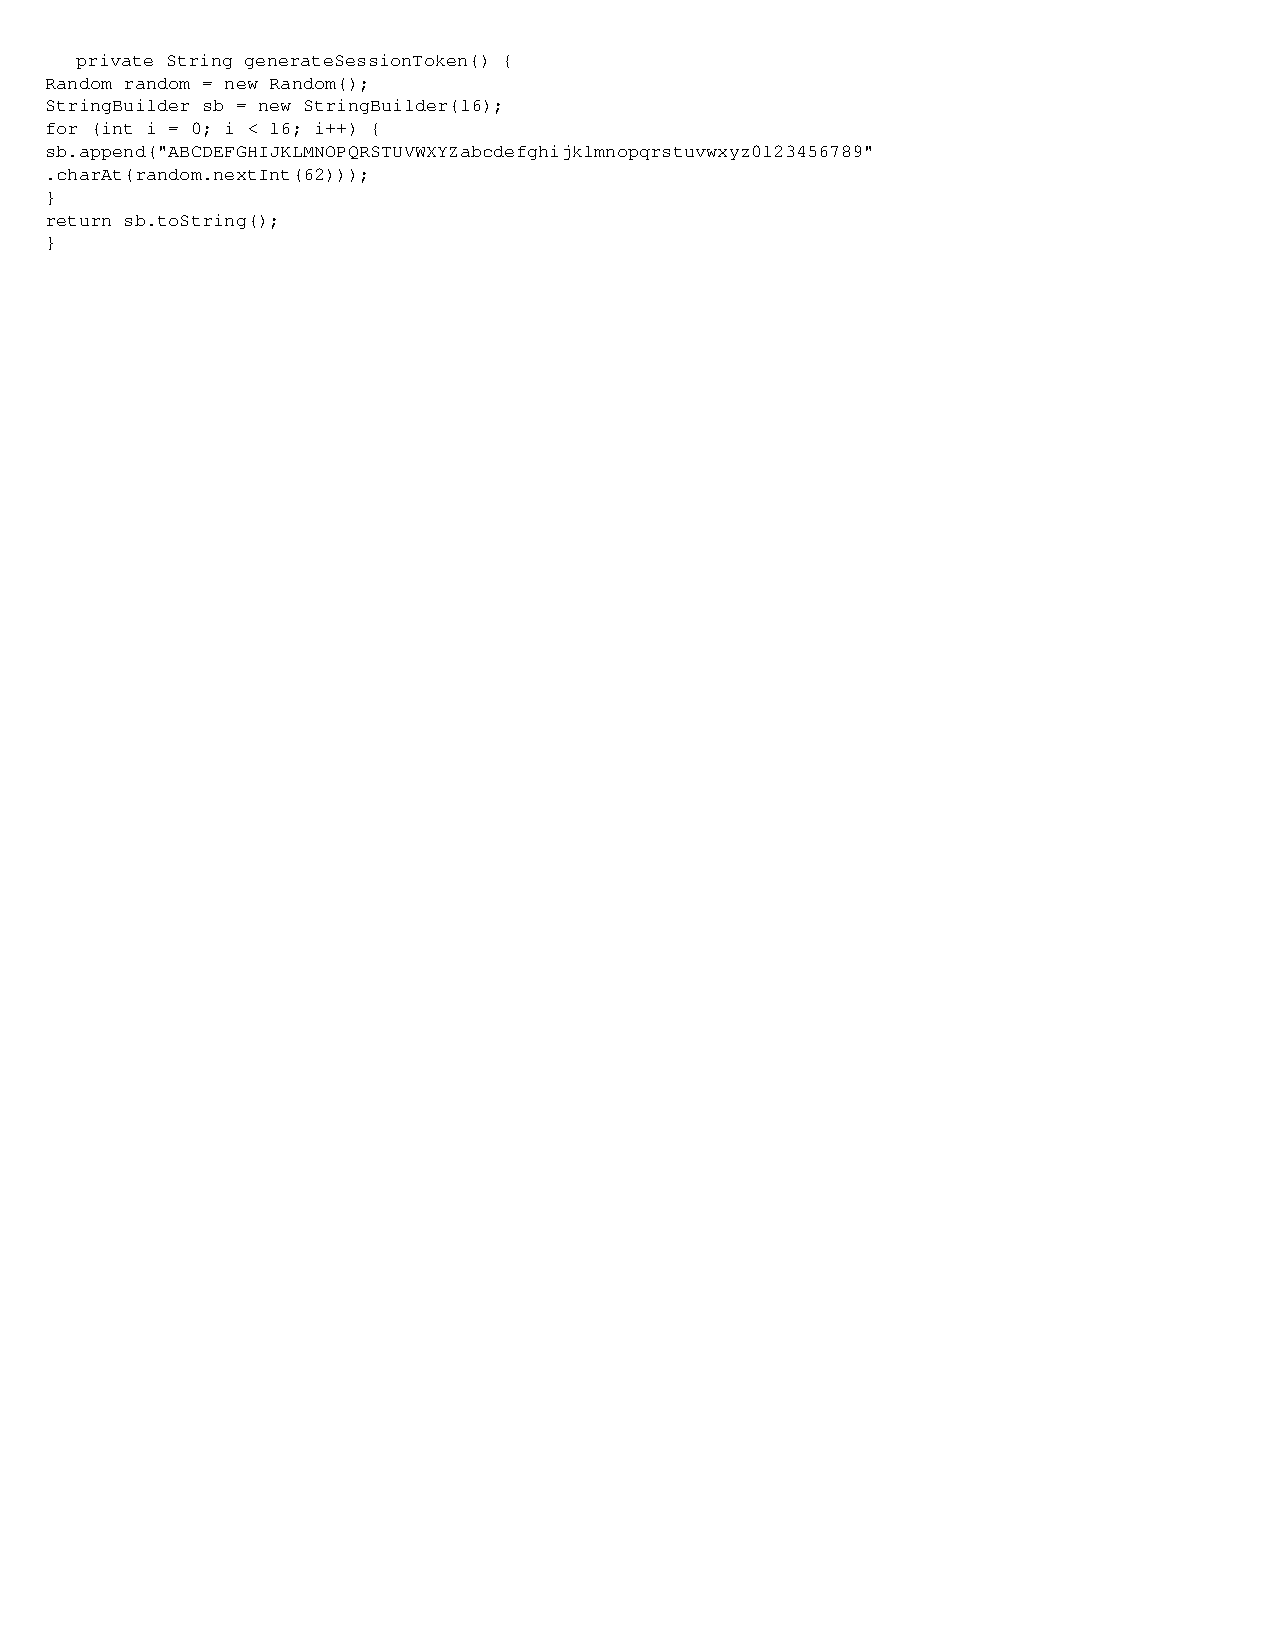
\includegraphics[width=\columnwidth]{figures/login_class_excerpt.pdf}
\caption{Excerpt of the decompiled session token generator from \texttt{Login.java}.}
\end{figure}

\section*{Vulnerability Details and Attack Path}
The core vulnerability is in \texttt{Login.generateSessionToken()}, where the app constructs a 16-character token from a fixed alphanumeric alphabet using \texttt{java.util.Random}. This API is a general-purpose pseudo-random number generator, not a cryptographically secure one. Its outputs are deterministic from internal state and therefore should not be used for authentication tokens, password reset codes, or keys.

The token is security-relevant because \texttt{Login.createSession()} writes \texttt{sessionToken} into \texttt{SharedPreferences}, and \texttt{Profile.clearSession()} later deletes the same value during logout. A realistic attack path is: (1) decompile the APK and recover the exact token generation algorithm; (2) observe when login occurs or collect one or more token outputs in a local test environment; (3) exploit the predictability of \texttt{Random} to reduce the internal state search space or predict future outputs; and (4) inject or reuse a predicted token to impersonate a valid session if the app or a future backend relies on this token for authentication. In the current code the session is only local, so the immediate impact is limited to local session integrity, but the design is already unsafe and would become more serious if reused in a backend-connected app.

\section*{Fix and Mitigation}
The fix is to replace \texttt{java.util.Random} with \texttt{java.security.SecureRandom} and generate at least 128--256 bits of entropy before encoding the result with Base64 or hexadecimal. For example, generate 32 random bytes with \texttt{SecureRandom.nextBytes()} and store the encoded value as the session token. This works because \texttt{SecureRandom} is designed to resist prediction, which is the exact failure mode of the current implementation. A stronger overall design would also enforce the token on protected screens and avoid storing plaintext credentials in \texttt{credentials.txt}.

\section*{References}
\begin{enumerate}[label={[}\arabic*{]}]
\item Oracle Java documentation for \texttt{java.util.Random}.
\item Oracle Java documentation for \texttt{java.security.SecureRandom}.
\item Android documentation for \texttt{SharedPreferences}.
\item Decompiled sources under \texttt{code/sources} and \texttt{code/resources}.
\end{enumerate}

\end{document}
